%\section{Asian GEM}
\label{chap:TPC_sec:asian_gems}
Contact person: Akira Sugiyama(email: sugiyama@cc.saga-u.ac.jp)\\

%\subsection{Engineering Challenges}

The Asian modules use GEM stacks as a gas amplification stage and are optimised to reduce the insensitive area
on the sides of the modules which point towards the detector center.
A module can be seen in figure \ref{fig_Fig1asiangempicture}.

\begin{figure}[!htb]
  \centering
  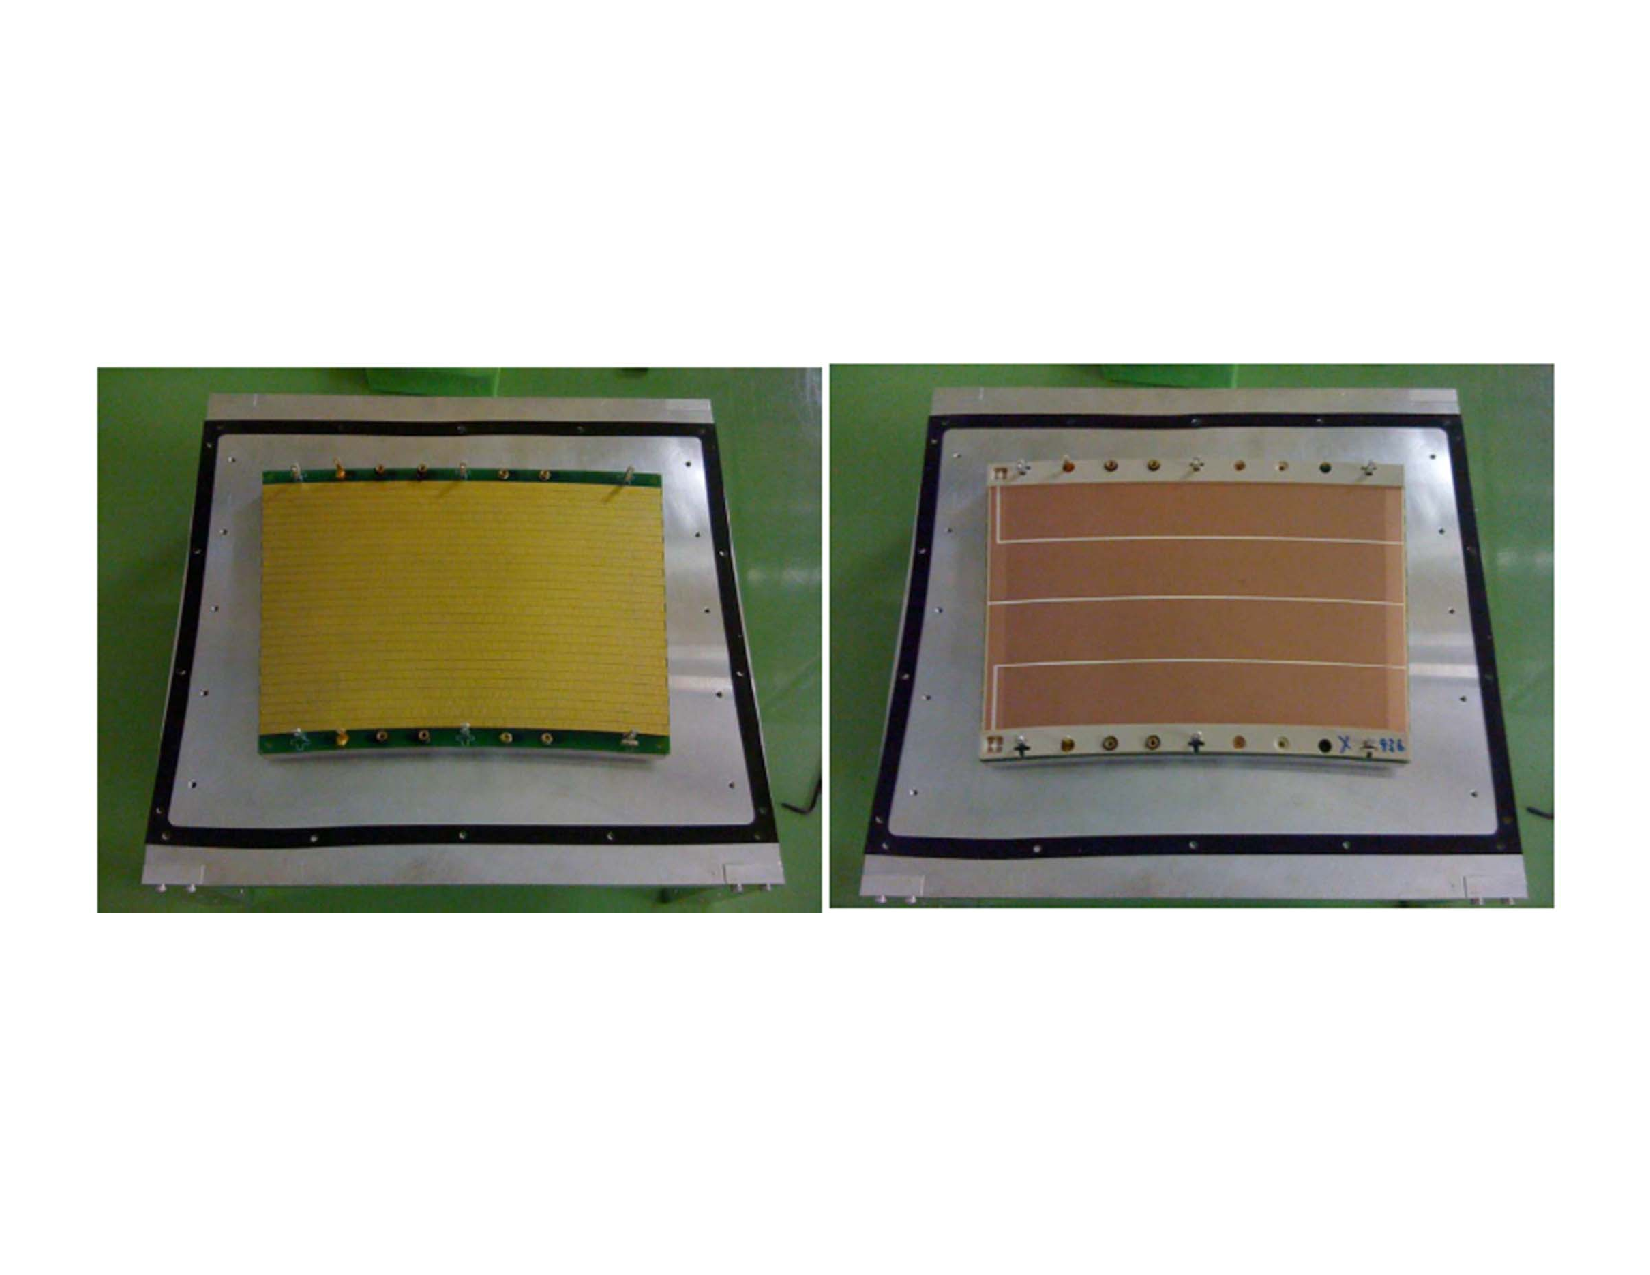
\includegraphics[width=0.9\textwidth]{Tracker/TPC_Bonn/plots/TPC-AG_Fig1asaingempicture.pdf}
  \caption{Asian GEM picture: left - anode pad plane; right - segmented cathode.}
  \label{fig_Fig1asiangempicture}
\end{figure}

Particles from the interaction point passing
between the modules may not be detected if they have very high momenta. Therefore, the Asian module foresees no frame along
the sides and extends the sensitive
area up to the edge of the backframe. To ensure a flat mounting of the GEMs, they are stretched on both the upper
and lower arcs (as seen in figure \ref{fig_Fig1asiangempicture}) which are made of a stiffer material:
GEMs with an insulator of \SI{100}{\micro\meter} Liquid Crystal Polymer (LCP)
covered with \SI{5}{\micro\meter} copper on both sides were produced by a company named SciEnergy.
The holes were
produced by \ce{CO2}-laser drilling after which they were carefully cleaned by dry etching to remove potentially
conductive residuals from the insides of the holes. The
hole pattern is identical to standard CERN GEMs. Because of the thicker material also higher gas gains per GEM
can be reached and a double GEM
structure is used and considered to be sufficient.
The two GEMs are mounted with an induction gap of \SI{2}{mm} and a transfer gap of \SI{3}{mm}.

The pad size is $1.2 \times \SI{5.4}{mm}$ and there are 28 pad rows with a total of 5152 pads.
From the beginning the use of an ion gate
(see subsection \ref{chap:TPC_sec:gating}) was envisaged and, thus, the level of the first GEM was designed
to be 1 cm below the nominal module height allowing for a later addition of the gate. To absorb the strength necessary
to stretch the GEMs and the gate, strong metal poles were implemented at the top and bottom arc.

\subsection{Recent Milestones}

All modules have been tested in the Large Prototype at DESY. The experience gained during all test beam periods as
well as the best transverse spatial resolution is described next. The testbeam measurements have used
the gas mixture of Ar-\ce{CF4}(3\%)-isobutane(2\%). The electric drift field was set in most cases to
E=\SI{230}{V/cm}, which is close to the maximum of the drift velocity, and alternatively to
E=\SI{130}{V/cm}, which is the minimum of the transverse diffusion.
The Asian modules were also measured using a laser system, in order to analyze the distortions.
The laser beam was scanned across the module, and the deviations were compared with calculations and are understood.

The Asian groups built three modules and made several test beam measurements at DESY (2009, 2010, 2012).
The first campaigns were dominated by very strong field distortions because of the mounting pins and the bare frames.
After introducing the field shaper, the distortions are comparable to the ones of other techniques used for modules.
The transverse spatial resolution is shown in figure \ref{fig_Fig2asiangemresolution}, where the measured spatial
resolution of a single row in the middle of a module can be seen.

\begin{figure}[!htb]
  \centering
  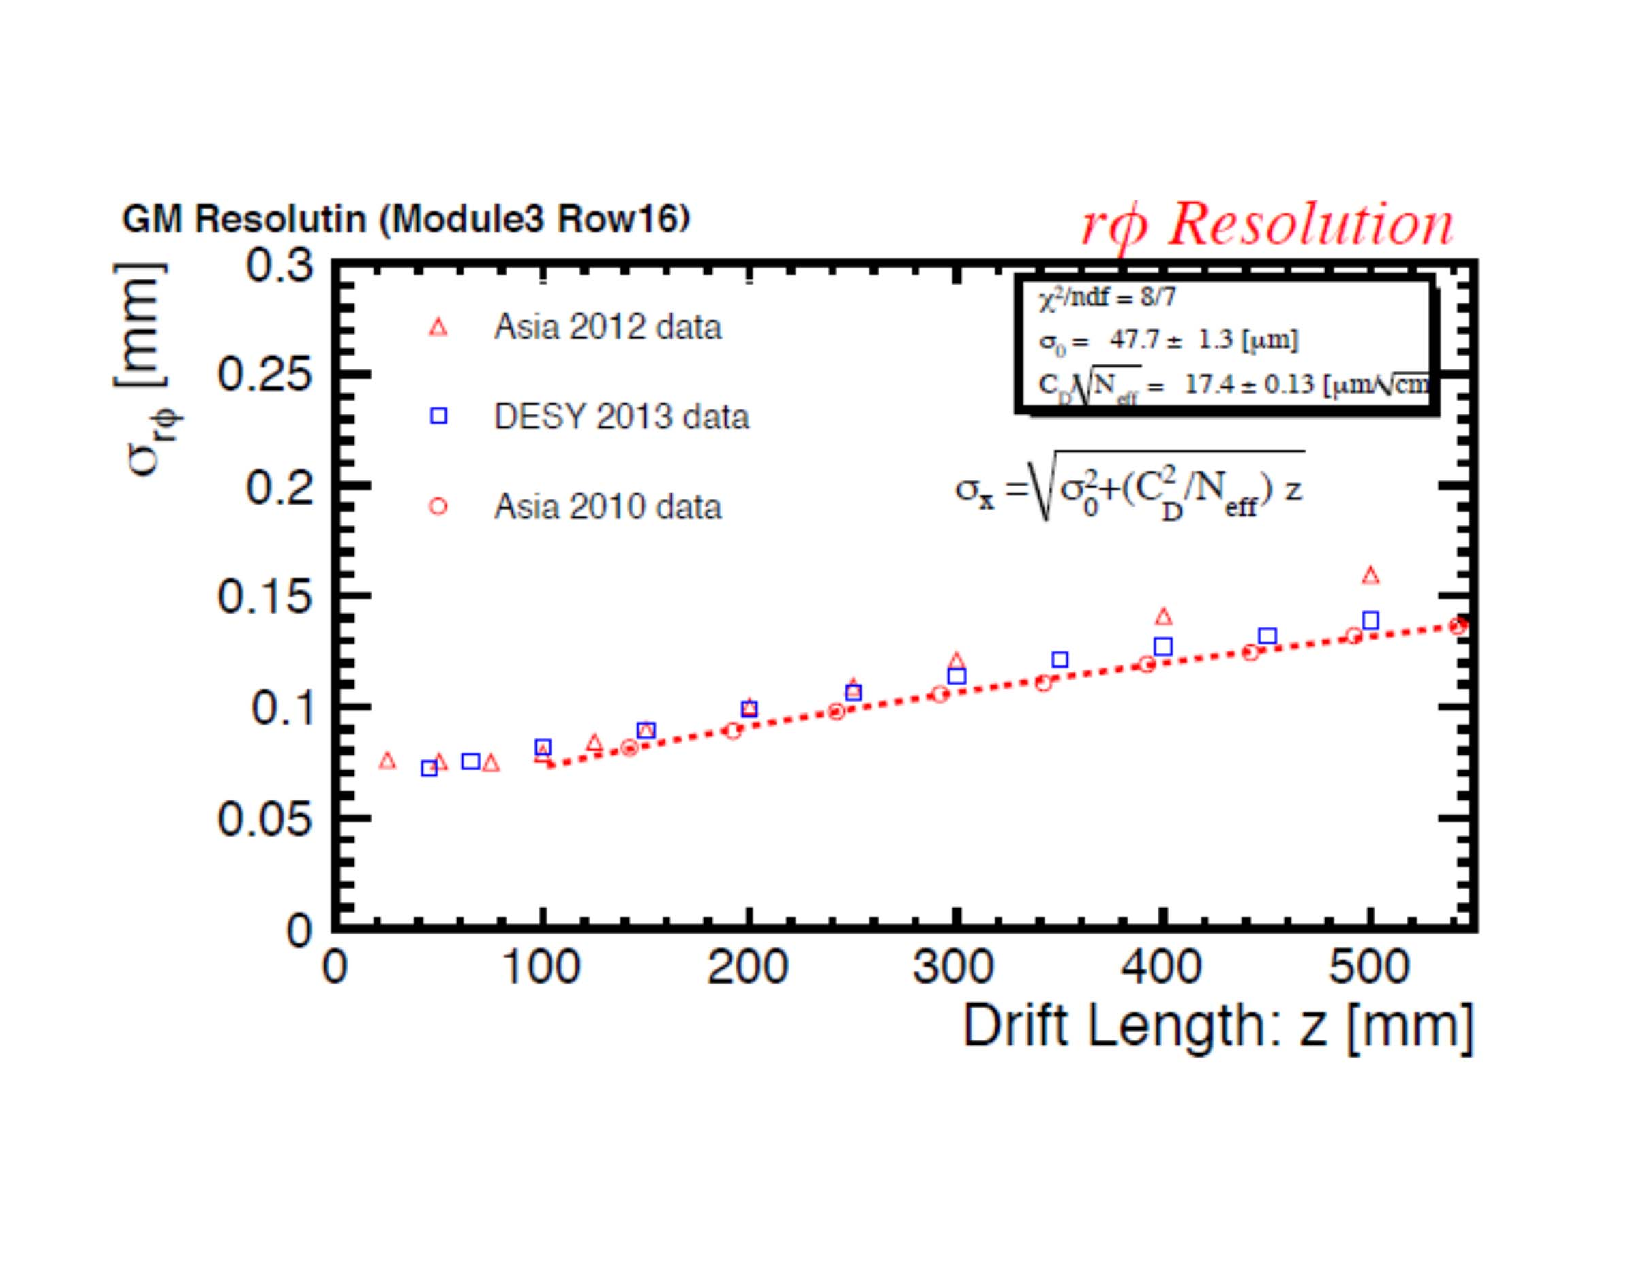
\includegraphics[width=0.9\textwidth]{Tracker/TPC_Bonn/plots/TPC-AG_Fig2asiangemresolution.pdf}
  \caption{Resolution measured for the Asian GEMs, and compared with a result for the DESY GEMs.}
  \label{fig_Fig2asiangemresolution}
\end{figure}

In this context an analytical formula was developed to predict the spatial resolution of a TPC. This formula includes
not only the effect of diffusion, angle,
noise and a finite pad-size, but also the influence of the electronics threshold, number of effective primary electrons,
the Polya-parameter of the gas
amplification, cross talk between pads and signal lines, charge loss because of attachment and the pad response function
are taken into account. All
these parameters can be varied and, if correctly chosen, describe well the measured data.

Finally, one other important observation was the HV micro-discharges on the Asian GEMs, with associated gain drops,
and investigations of this problem are summarized here.

To minimize the energy released in a discharge, the GEMs were segmented into four arcs, each with an area of
about $\SI{100}{cm^2}$ (figure \ref{fig_Fig1asiangempicture}, right).
Studies of the micro-discharges for the various types of GEMs were measured under a controlled environment.
The \SI{100}{\micro\meter} Asian GEMs discharged frequently, while the DESY \SI{50}{\micro\meter} GEMs (made by CERN) had little or no
discharges. For the \SI{50}{\micro\meter} GEMs, there is no significant difference of
the discharge rate between different types of GEMs. It is noteworthy that, at low gain, the \SI{100}{\micro\meter} GEMs
had a discharge rate which is almost the same as for the \SI{50}{\micro\meter} GEMs. The water content in the gas does not seem to
influence the
discharge rate, and long-term measurements are in progress.


\subsection{Future Plans}

In the future, it is planned to:\\
$\bullet$ understand better the reasons for the micro discharges and eliminate them, and \\
$\bullet$ construct a full scale Asian module with gate.
